

\tikzset{every picture/.style={line width=0.75pt}} %set default line width to 0.75pt

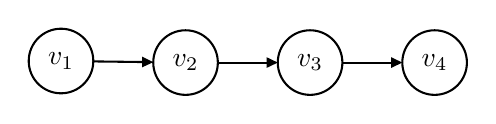
\begin{tikzpicture}[x=0.75pt,y=0.75pt,yscale=-1,xscale=1]
%uncomment if require: \path (0,66); %set diagram left start at 0, and has height of 66


% Text Node
\draw    (40, 30.25) circle [x radius= 15.56, y radius= 15.56]   ;
\draw (40,30.25) node   [align=left] {\begin{minipage}[lt]{13.600000000000001pt}\setlength\topsep{0pt}
\begin{center}
$\displaystyle v_{1}$
\end{center}

\end{minipage}};
% Text Node
\draw    (100, 31) circle [x radius= 15.56, y radius= 15.56]   ;
\draw (100,31) node   [align=left] {\begin{minipage}[lt]{13.600000000000001pt}\setlength\topsep{0pt}
\begin{center}
$\displaystyle v_{2}$
\end{center}

\end{minipage}};
% Text Node
\draw    (160, 31) circle [x radius= 15.56, y radius= 15.56]   ;
\draw (160,31) node   [align=left] {\begin{minipage}[lt]{13.600000000000001pt}\setlength\topsep{0pt}
\begin{center}
$\displaystyle v_{3}$
\end{center}

\end{minipage}};
% Text Node
\draw    (220, 31) circle [x radius= 15.56, y radius= 15.56]   ;
\draw (220,31) node   [align=left] {\begin{minipage}[lt]{13.600000000000001pt}\setlength\topsep{0pt}
\begin{center}
$\displaystyle v_{4}$
\end{center}

\end{minipage}};
% Connection
\draw    (55.56,30.44) -- (81.45,30.77) ;
\draw [shift={(84.44,30.81)}, rotate = 180.72] [fill={rgb, 255:red, 0; green, 0; blue, 0 }  ][line width=0.08]  [draw opacity=0] (5.36,-2.57) -- (0,0) -- (5.36,2.57) -- cycle    ;
% Connection
\draw    (115.56,31) -- (141.44,31) ;
\draw [shift={(144.44,31)}, rotate = 540] [fill={rgb, 255:red, 0; green, 0; blue, 0 }  ][line width=0.08]  [draw opacity=0] (5.36,-2.57) -- (0,0) -- (5.36,2.57) -- cycle    ;
% Connection
\draw    (175.56,31) -- (201.44,31) ;
\draw [shift={(204.44,31)}, rotate = 540] [fill={rgb, 255:red, 0; green, 0; blue, 0 }  ][line width=0.08]  [draw opacity=0] (5.36,-2.57) -- (0,0) -- (5.36,2.57) -- cycle    ;

\end{tikzpicture}